\documentclass{mpaper}
\usepackage{multirow}
\usepackage{subcaption}

\begin{document}

\title{Is Technical Debt Real?}
\author{Ovidiu Popoviciu}
\matricnum{2036725p}


\maketitle


\begin{abstract}
The concept of technical debt has received considerable attention in recent
years in both research and industry. Despite this, there is relatively little
empirical evidence as to the longer term impact of technical debt on a software
project. In our work, we seek to test the hypothesis that technical debt incurs
work-effort `interest' in a software project, arising through increased feature
implementation costs. In this paper, we test the correlation between technical
debt and work effort by measuring the cost of implementation of a work item
within five project histories and measuring the impact of technical debt on
implementation cost. It is hoped that this study is the first step in a series
on identifying technical debt and on provisioning of a decision-support method
to enable software project teams to make rationale long-term decisions as to the
management of quality issues. 
\end{abstract}

%%%%%%%%%%%%%%%%%%%%%%%%%%%%%%%%%%%%%%%%%%%%%%%%%%%%%%%%%%%%%%%%%%%%%%%%%%%%%%%
%%%%%%%%%%%%%%%%%%%%%%%%%%%%%%%%%%%%%%%%%%%%%%%%%%%%%%%%%%%%%%%%%%%%%%%%%%%%%%%
%%%%%%%%%%%%%%%%%%%%%%%%%%%%%%%%%%%%%%%%%%%%%%%%%%%%%%%%%%%%%%%%%%%%%%%%%%%%%%%
\section{Introduction}
\label{introduction}

\begin{enumerate}
  \item General description of the problem, motivation, relevance
  \item Contributions to state of the art 
  \item Research questions
  \item Section descriptions
\end{enumerate}

Research questions:

Is there any correlation between technical debt and work effort?
Does work effort increase when technical debt is added?
Does work effort decrease when technical debt is removed?

Is there a correlation between technical debt and change set size?
Do less changes mean that technical debt is introduced?
Do more changes mean that technical debt was removed? 


% The precise structure of an MSci paper is not mandated, but it should probably
% cover in detail the following aspects of the project. \begin{enumerate} \item
% General description of the problem, motivation, relevance \item Background
% information, possibly including a literature survey \item Description of
% approach taken to solve the problem, including high-level design and
% lower-level implementation details as appropriate \item Evaluation,
% qualitative or quantitative as appropriate \item Conclusion, including scope
% for future work \end{enumerate}

%%%%%%%%%%%%%%%%%%%%%%%%%%%%%%%%%%%%%%%%%%%%%%%%%%%%%%%%%%%%%%%%%%%%%%%%%%%%%%%
%%%%%%%%%%%%%%%%%%%%%%%%%%%%%%%%%%%%%%%%%%%%%%%%%%%%%%%%%%%%%%%%%%%%%%%%%%%%%%%
%%%%%%%%%%%%%%%%%%%%%%%%%%%%%%%%%%%%%%%%%%%%%%%%%%%%%%%%%%%%%%%%%%%%%%%%%%%%%%%
\section{Background}
\label{background}

There are a number of studies which have investigated the impact of technical
debt items on the costs of software projects.  This section reviews this work
and relates the existing state of the art to our proposed experiment to
empirically measure the work effort interest accumulated by technical debt.

Olbrich et al. \cite{Olbrich2009} studied the impact of two code smells, God
class and Shotgun Surgery, on change-proneness of class entities and size of
changes within two open source systems, Apache Lucene and Apache Xerces. They
found that classes containing either smell are more change prone than other,
non-smelly, classes. In a similar study, Khomh et al. \cite{Khomh2009}
empirically analysed the impact of 29 code smells on the change-sets of 9
releases of two open source systems. They had confirmed the results of the
previous studies that code smells increase the number of changes that software
undergoes during its evolution. Additionally, they had found that classes
containing more than one code smell are more change prone than other classes.
Charalampidou et al. \cite{Charalampidou2017} introduced a study that assessed
the interest probability of code smells, which is the probability of a code
smell to introduce extra changes in future development. Interest probability was
calculated by counting the frequency of each code smell and how it correlated
with the change-proneness of the module where it resides. The smells studied
were Long Method, Conditional Complexity and Duplicated Code. The results showed
that code duplication had the highest interest probability due to the number of
changes required to maintain future development. Additionally, high cyclomatic
method complexity increased the number of changes. Fontana et al.
\cite{Fontana2012} studied what was the impact of removing code smells on code
quality metrics such as cohesion, coupling and complexity and, which smell
incurred the most debt. They applied refactoring activities for each smell and
the metrics were re-evaluated. The results showed that refactoring of one code
smell might provide benefits for some metric qualities but may negatively impact
others.

The authors studied the impact of code smells and their removal on the software
quality metrics output by directly analysing reports of code quality tools.
Although their research has increased awareness of technical debt, our proposed
work aims to focus on what impact quality issues and bug patterns have on work
effort implementation by measuring the work effort involved. Additional studies
have looked at quantifying implementation cost in the context of technical debt.

Singh et al. \cite{Singh2014}, calculated interest payments by monitoring
development effort and code comprehension. They monitored time spent by
developers in classes with known technical debt items and implemented a tool
within the Integrated Development Environment of developers to gather
information on class visits and development session times. The interest was
quantified as the difference between time practically spent in classes and the
ideal time. However, the study was conducted with the input of only one
developer over a period of 9 months. Additionally, estimating the ideal time
spent on development is a challenging task due to social and personal factors
such as level of project knowledge, environment familiarity and programming
language preference.

Gomes et al. \cite{Gomes2011} studied the correlation between software
evolution, defect occurrence and work effort deviation at the release level. The
authors extracted data from documentation sources such as test plans, project
plan, weekly reports, project source code, and emails. Using this data, they
could derive important team information on change-sets, effort, quality, test
and size of the system. They measured extra work effort by subtracting the
estimated work time and total practical work time. Although information at the
release level offers project managers an idea of work effort deviation, it does
not show at a granular level what defects slow down development of a new feature
and where the team should focus their refactoring activities.

The initial study by Gomes et al. \cite{Gomes2011} provided a good start to
identifying work effort deviation. However, it only analysed major releases of a
system and did not provide drill-down information on iterations and code commits
on which features and code smells had the most effect on work effort. This is
essential information for developers and project managers to prioritise
refactoring activities in work iterations, especially in an Agile environment
where responding to change is critical \cite{agile-manifesto}.

%%%%%%%%%%%%%%%%%%%%%%%%%%%%%%%%%%%%%%%%%%%%%%%%%%%%%%%%%%%%%%%%%%%%%%%%%%%%%%%
%%%%%%%%%%%%%%%%%%%%%%%%%%%%%%%%%%%%%%%%%%%%%%%%%%%%%%%%%%%%%%%%%%%%%%%%%%%%%%%
%%%%%%%%%%%%%%%%%%%%%%%%%%%%%%%%%%%%%%%%%%%%%%%%%%%%%%%%%%%%%%%%%%%%%%%%%%%%%%%
\section{Methodology}
\label{methodology}

In this paper, we present an approach for aggregating development team data
sources such as project management tools, version control logs and static
analysis results to produce a timeline of technical debt and work effort over
the evolution of a software product. Our motivation is to empirically find a
correlation between technical debt and the amount of work effort involved in
development of work items. In the absence of work tracking information,
aggregation of such data sources might provide a relatively accurate estimation
of the number of hours a developer has put in.

When developing our approach, we completed the following steps:
\begin{enumerate}
  \item Designing an initial data model.
  \item Selecting data candidates (projects) that satisfy specific criteria.
  \item Collecting data from issue tracker, version control logs and generating
  static analysis output.
  \item Processing and refining data for analysis. 
\end{enumerate}

Section \ref{experimental-design} dives into the data model while section
\ref{data-selection} describes the data candidates criteria and selected
projects. The data collection process is described in Section
\ref{data-collection} while the calculation of work effort and technical debt is
described in Section \ref{data-processing}.

% - - - - - - - - - - - - - - - - - - - - - - - - - - - - - - - - - - - - - - -
\subsection{Experimental Design}
\label{experimental-design}

The initial step was to design a model of the aggregated data and to understand
what type of information each selected data source will provide. We consider the
following data sources relevant to the collection of data:

\begin{itemize}
  \item A \emph{Version Control System} is a system that manages changes to the
  source code. As work items are implemented, the system logs all changes made
  by the development team. The most popular version control tool is Git
  \emph{REFERENCE}. GitHub \emph{REFERENCE} and BitBucket \emph{REFERENCE} are
  hosting services for source code management.

  \item \emph{Project Management Tools} are software systems that help teams
  track, manage and collaborate on various types of units of work. A common
  example of a complex project management tool is Jira \emph{REFERENCE}. GitHub
  and BitBucket also provide an issue tracking tool with each code repository,
  although they do not provide such extensive features as Jira.
  
  \item \emph{Static Analysis Tools} are tools that analyse the source code to
  check for quality issues, security flaws and adherence to industry
  standards.There are many examples of static analysis tools: SonarQube,
  Spotbugs (formerly Findbugs), CAST, Sonargraph, etc.

\end{itemize}

All the data sources contain detailed information related to the set of changes
that the source code has suffered, the requirement that the developer is working
on and the possible quality issues she will encounter during implementation. In
many cases, these systems have been implemented by different producers and thus
are generally ``separated''. Therefore, data must be collected from each system,
in isolation. However, forms of ``light integrations'' exists for development
productivity purposes such as linking of work items to change-sets by specifying
the work item ID in the change-set description message. Such provide guidance on
how many change-sets the source code has suffered during the implementation of a
work item.

The centralised data model, presented in Figure \emph{FIGURE}, highlights the
integration of version control logs, issue tracker data and static analysis
output. The next few sections highlight the data model of each source in
isolation.

% - - - - - - - - - - - - - - - - - - - - - - - - - - - - - - - - - - - - - - -
\subsubsection*{Version Control}
\label{version-control}

The version control system keeps track and logs all changes that a source code
has suffered over the evolution of the product. Such logs are indispensable due
to their metadata which provides information on the accomplished work.

Git \emph{REFERENCE} is a popular version control tool that tracks changes of
the source code using branches and commits. Projects are stored in a
``repository'' which contains at least one development line, called a
``branch''. The main development branch is commonly named the \emph{master}
branch. Branches contain a stream of small units of work, called ``commits'',
which are the snapshots of the source code at a particular point in time.
Additionally, each commit contains relevant metadata with the following fields:

\begin{itemize}
  \item \emph{Object ID} - is the identifier of the snapshot;
  \item \emph{Author} - the name (or username) of the developer that committed
  the change;
  \item \emph{Message} - a short description of the change-set;
  \item \emph{Timestamp} - the time when the commit was created;
  \item \emph{Diff} - the set of changes that the source code has suffered, when
  compared to the previous commit. 
\end{itemize}

If the system allows integrations with a project management tool, changes can be
directly linked to the appropriate work unit. The most common method is to
specify the work item ID in the message field of the commit ID. As a result, it
is simpler to find out which change-sets belong to a particular work item. 

For a project managed using Git, all the metadata can be easily retrieved and
snapshots can be accessed at any time. This makes Git a powerful tool in
studying the history of changes of a software product.

% - - - - - - - - - - - - - - - - - - - - - - - - - - - - - - - - - - - - - - -
\subsubsection*{Project Management}
\label{project-management}

Project management tools allows developers and project managers to keep track of
the work that must be accomplished and of the issues that have been reported by
the users of the software. 

Each work item is represented in the form of a \emph{ticket}, which is a report
of the work that needs to be completed. Depending on the workflow of the team,
tickets may go through various status transitions during their lifetime which
represent checkpoints of the work involved. A ticket may contain a lot of data,
including but not limited to:

\begin{itemize}
  \item \emph{ID} - the unique identifier of the work item in the project;
  \item \emph{Type} - the type of work e.g. Feature, Bug, Enhacement, etc.;
  \item \emph{Status} - the current status of the work e.g. Created, In
  development, In testing, Closed, etc.;
  \item \emph{Summary} - a brief description of the work;
  \item \emph{Description} - a longer, more detailed description of the work
  involved;
  \item \emph{Priority} - the importance of the work as considered by the team;
  \item \emph{Assignee} - the team member responsible for completing the work;
  \item \emph{Complexity} - measurement of how complex the work item is e.g.
  Story points;
  \item \emph{Comments} - a list of comments by other team members to promote
  discussion on the work;
  \item \emph{Timestamps} - the times when ticket was created, updated, closed
  and when it is due. 
\end{itemize}

Additionally, Jira tickets contain a field called \emph{Time Tracking} that
allows tracking of the estimated time to complete the work, time logged and time
left. Moreover, for Jira, the history of changes of a work item is available
through its API in a field called \emph{Transitions}. This metadata provides a
good idea of when development for a specific work has started or ended, by
analysing the changes of the status field over time. 

Although project management tools provide relevant work tracking information,
not all tools offer the same broad scope of work data. For example, the
integrated issue tracker within GitHub and BitBucket do not offer the same
features and functionality that Jira does. Additionally, many of the fields of
tickets might be non-existent. This poses a problem to the validity of the work
effort calculations, mentioned in section \ref{data-processing}. 

% - - - - - - - - - - - - - - - - - - - - - - - - - - - - - - - - - - - - - - -
\subsubsection*{Static Analysis}
\label{static-analysis}

% intro
Static analysis tools provide an elegant method of analysing source code for
possible weaknesses and quality issues without a direct execution of the entire
product. Its applicability makes it a great tool for developers to analyse their
change-sets at any time of the implementation process.

% body
The output of static analysis tools are generally weaknesses and bugs that may
lead to vulnerabilities which are considered ``lowest level'' of technical debt.
Code debt is technical debt that developers have to encounter daily
\emph{REFERENCE}. There are many static analysis tools, many of which have been
reviewed \emph{REFERENCE}, \emph{REFERENCE}. 

Although static analysis tools provide an approximate measure of the quality of
the code base, there is a danger in associating technical debt with their
output. There are multiple types of technical debt present in the software
development environment \emph{REFERENCE}. For example, static analysis tools
cannot predict that the requirements gathering phase was not completed
appropriately and thus it might take more time for a team member to understand
the expectations of a work item, thus indirectly increasing effort. However, as
a simplifying assumption, in this paper we only consider code debt in the
calculation of a technical debt index. 

The output of a static analysis tool that we are interested in contains the
following fields:

\begin{itemize}
  \item \emph{ID} - a unique identifier of the quality issue;
  \item \emph{Priority} - a generic measure of severeness e.g. High, Medium,
  Low;
  \item \emph{Description} - a short description of the code violation;
  \item \emph{Location} - the location of the quality issue, represented by the
  file name and line number. 
\end{itemize}

This type of output gives a representation of the possible low-level weaknesses
that developers might introduce and encounter during the implementation process.
Additionally, by using the version control logs it is possible to track the
items that have been introduced or removed for each change-set as well as the
total amount of issues that a team member had to deal with. 

Unfortunately, not all projects use a static analysis tool to check for issues
and, if some do, they are not publicly available in a centralised system as well
as not being available for each revision of the source code. This challenge was
addressed and is described in section \ref{data-collection}. 

% - - - - - - - - - - - - - - - - - - - - - - - - - - - - - - - - - - - - - - -
% - - - - - - - - - - - - - - - - - - - - - - - - - - - - - - - - - - - - - - -
% - - - - - - - - - - - - - - - - - - - - - - - - - - - - - - - - - - - - - - -
\subsection{Candidates selection}
\label{data-selection}

% intro
For the purpose of this experiment, we had to apply the data collection
processing phases on a set of software projects. These projects had to satisfy a
certain criteria to be included:

\begin{itemize}
  \item Use \emph{Git} as a version control tool due to its powerful features,
  applicability and popularity. Additionally, the project must be open-source to
  access the history of snapshots.
  \item Use a project management tool that is publicly accessible to retrieve
  work item data.
  \item Use \emph{Java} as the main programming language. This was a simplifying
  criteria to keep the data collection and processing consistent. Additionally,
  this aided our decision in selecting a single static analysis tool.
  \item The project should have a single main development branch, preferably the
  ``master'' branch. This relieves the data collection process of analysing
  multiple branches.
  \item The version control hosting system should integrate with the project
  management tool to highlight the commits that belong to a specific work item.
  \item The project uses Maven as its build system due to simplifications in
  development process of the data collection tool. Multiple build systems could
  be added if necessary.
\end{itemize}

\begin{table}
	\begin{tabular}{|l|r|c|}
    \hline
		\emph{Project Name}        & \emph{Size (LOC)} & \emph{Issue Tracker}  \\ \hline \hline
		ANTLR                      & 399,388            & GitHub               \\ \hline
		Spring HATEOAS             & 25,601             & GitHub               \\ \hline
		Checkstyle                 & 353,273            & GitHub               \\ \hline
		Apache Commons Collections & 124,854            & Jira                 \\ \hline
		Apache Commons Lang        & 158,713            & Jira                 \\ \hline
	\end{tabular}
	\caption{\label{tab-data-candidates} Data candidates}
\end{table}

% body 
Table \ref{tab-data-candidates} shows the selected open-source projects that have their data
collected and analysed as well as their size (LOC), version control and project
management tools. Out of the ten projects, we have only included five for
analysis of results due to an incomplete data collection process. This was a
result of:

\begin{itemize}
  \item Unavailable APIs for accessing project management tool.
  \item Non-existent static analysis output. This might be due to a ``Zero
  Bugs'' policy set by the development team.
  \item Failing build process for the majority of revisions. The build process
  was failing on too many revisions to provide any meaningful data.
\end{itemize}

Since the projects selected for this experiment are managed by different
development teams, some of the data sources are distributed and use different
underlying technologies. Additionally, not all projects make use of a static
analysis tool and therefore such data might not be publicly available. As a
result, we have decided to execute static analysis on each revision of the main
branch our candidate projects. This brings the advantage of a consistent data
model of quality issues and fills in the void left by the lack of static
analysis data. However, this decision introduced an additional overhead in the
data collection process.

% - - - - - - - - - - - - - - - - - - - - - - - - - - - - - - - - - - - - - - -
% - - - - - - - - - - - - - - - - - - - - - - - - - - - - - - - - - - - - - - -
% - - - - - - - - - - - - - - - - - - - - - - - - - - - - - - - - - - - - - - -
\subsection{Data collection}
\label{data-collection}

% intro
To collect the selected data from multiple systems we built a tool that
retrieves data from each source and centralises them into a single database for
processing and analysis. Additionally, this method allows us to reproduce the
experiment without any outside changes to the dataset while future work items do
not incur an additional data collection overhead. Moreover, due to the choice of
database technology, new data could be added from additional projects without
any changes to the initial data model. Figure \emph{FIGURE} shows a simple view
of the data model.

The tool has been built using Java and open-source technologies, and is
available to use by anyone (MIT License) \emph{REFERENCE}. The tool uses the
following technologies for collecting data:

\begin{itemize}
  \item jGit \emph{REFERENCE} - is a Java library for interacting with the Git
  version control system;
  \item REST Java Client for Jira \emph{REFERENCE} - is a Java library that
  provides a simple interaction with Jira APIs;
  \item GitHub API for Java \emph{REFERENCE} - is a Java library that provides
  integration with GitHub API for retrieving issues;
  \item MongoDB \emph{REFERENCE} - NoSQL database technology for storing
  collected data;
  \item Spotbugs \emph{REFERENCE} - tool for identifying bug patterns in source
  code;
  \item Other technologies - Spring Boot \emph{REFERENCE}, Angular \emph{REFERENCE} and ChartJS \emph{REFERENCE}
  for visualising data.
\end{itemize}

The data collection process is shown in figure \emph{FIGURE}. Firstly, selected
project repositories are cloned to the local storage. Secondly, the tool starts
the ``collection step'', where each revision of the project history is processed
serially, starting with the latest revision and going back in time. The
collection step is composed of multiple sub-steps:
\begin{enumerate}
  \item \emph{Retrieve commit metadata}.
  \item \emph{Search and retrieve ticket(s)}. The current commit message is
  analysed for mentions of ticket IDs. For any ticket ID found, the tool
  retrieves the ticket from the project management tool API.
  \item \emph{Build current revision}. This is a preparation step for the static
  analysis. The source code of the project must be compiled into classes and
  packaged into JARs for static analysis to complete.
  \item \emph{Statically analyse the JARs}. Scan the current revision JARs for
  quality issues. If the build process fails, then the static analysis scan is
  skipped, due to missing JAR files. 
\end{enumerate}

Data is stored at the end of each substep to avoid an inconsistent commit stream
in case one of the next one fails or the tool crashes.

During development, the building and static analysis steps incurred an extreme
overhead that was slowing down the data collection process. For a repository
with thousands of revisions, there would have been a significant time overhead
that would overstep the timeline of the experiment. Therefore, the build process
was customised by skipping a few unnecessary tasks that we did not consider in
scope for this experiment:

\begin{itemize}
  \item Generating of documentation;
  \item Compiling and running tests;
  \item Test coverage checks;
  \item Integrated code analysis.
\end{itemize}

Some projects had an integrated static analysis task as part of the build
process. We decided to skip it due to the implementation of the Spotbugs
analysis step and due to complexities in the integration with multiple analysis
tools. 

Additionally, the tasks that compile and run the testing suites were ignored.
Firstly, testing was considered a separate activity to the implementation of new
features, fixing bugs and adding enhacements. Thus, in this case, code debt was
split into ``implementation debt'' and ``testing debt''. Testing debt refers to
shortcuts taken during the testing phases \emph{REFERENCE}. Secondly, the
testing task added an additional overhead to the build process. In reality,
testing is a fundamental part of development and is tightly integrated with
implementation of work items, especially in the practice of Test Driven
Development. It is one of the top most mentioned type of technical debt in a
mapping study by X et. al \emph{REFERENCE}, along with code, architecture and
design debt. The integration of testing debt within this experiment is
considered as a future work item, mentioned in section \ref{future-work}.

\begin{table*}[t]
	\centering
	\begin{tabular}{|l|r|r|r|r|r|}
		\hline
		Category                & \emph{ANTLR} & \emph{Spring HATEOAS} & \emph{Checkstyle} & \emph{Commons Collections} & \emph{Commons Lang} \\ \hline \hline
		Total Commits           & 728          & 539                   & 1,814             & 3,306                      & 5,061               \\ \hline
		Total Tickets           & 215          & 173                   & 188               & 236                        & 304                 \\ \hline
		Build Successful        & 478          & 472                   & 1,732             & 392                        & 3,814               \\ \hline
		Build Failed            & 250          & 67                    & 82                & 2,914                      & 1,247               \\ \hline
		Commits with Tickets    & 217          & 327                   & 1,157             & 437                        & 1,306               \\ \hline
		Commits without Tickets & 511          & 212                   & 657               & 2,869                      & 3,755               \\ \hline
		Ticket / Commit         & 0.217        & 0.744                 & 0.654             & 0.034                      & 0.258               \\ \hline
	\end{tabular}
	\caption{\label{tab-data-collection} Data collection results}
\end{table*}


% conclusion
The results of the data collection is shown in Table \ref{tab-data-collection}.
Although only \emph{N} projects have been selected out of the initial 11
presented in section \ref{data-selection}, using our data collection process we
have managed to retrieve and analyse \emph{M} commits and \emph{X} issues along
with an average of \emph{T} unique quality issues. Additionally, this process
was repeated a second time due to changes in the static analysis collection
step. Section \ref{results-discussion} dives into the results of our analysis. 

% - - - - - - - - - - - - - - - - - - - - - - - - - - - - - - - - - - - - - - -
\subsection{Data processing}
\label{data-processing}

% intro
Although, the collection step gathered data from three systems and stored them
into a single source of truth, in its current state it could not have been used
to derive any meaningful information on the correlation between technical debt
and work effort. Therefore, a ``processing stage'' was implemented in the tool,
that allows the calculation of these metrics and visually displays statistics on
using charts.

% body
The processing stage revolved around the concept of work items (WI). Work items
are pieces of work assigned to developers of the project. Each item is composed
of a ticket (T) and a list of commits (C), ordered chronologically. Tickets
represents the pieces of data retrieved from the project management tool. The
list of commits represent a subset of the total revisions of the repository that
belong to that specific work item. As mentioned in section
\ref{data-collection}, commits are assumed to belong to a specific ticket if
their commit message actively references the ticket ID of the project management
tool.

The work items can be deduced from the data collected. However, there are two
fundamental measures which must be derived:
\begin{itemize}
  \item Work effort (WE) - the total number of man-hours put in for a specific
  work item;
  \item Technical Debt (TD) - the total number of technical debt items that have
  affected the work at the time of implementation.
\end{itemize}

% - - - - - - - - - - - - - - - - - - - - - - - - - - - - - - - - - - - - - - -
\subsubsection*{Work Effort}
\label{work-effort}

% calculation of work effort
As mentioned, the work effort is the total number of hours put in by a single
developer towards the design and implementation of a work item. For simplicity,
we considered that an item of work followed a linear pattern and that a
developer was working on a single work item at a time.

From this assumption, we considered that each work item has a start time ($t1$)
and end time ($t2$), both expressed as timestamps in Greenwich Mean Time (GMT)
format. A simple method for calculating the work effort is to take the
difference between these two timestamps. This makes it easy to calculate the
working hours on the same day:

\begin{equation}
  \label{eq-work-effort-simple}
  WE = hours(t1 - t2)
\end{equation}

For example, if a developer starts work on a task on Monday at 9:00 GMT and
finishes work at 15:00 GMT, then the total of effort put in for that task is 6
hours. However, a work item might span multiple days and thus this solution
would include hours outside hours. To cover for this case, we introduced another
simplyfing assumption. Assume that the normal working hours per day would not
exceed 8 hours. This means that work spread over multiple days would be
calculated as follows:

\begin{equation}
  \label{eq-work-effort-days}
  WE = (days(t1 - t2) + 1) * 8
\end{equation}

If the work spans multiple days, then the total effort is the total number of
days multiplied by the number of working hours per day. For example, let's
assume that a developer starts a work item on Monday, 9:00 GMT and finishes his
work on Tuesday, 21:00 GMT. This equation will yield 16 hours of work spanning
two days (Monday and Tuesday). We recognize that there are multiple factors that
affect the work effort put in for a work item which are not modelled as part of
the calculation. These two equations were chosen for their simplicity and to
match the type of data at disposal. 

From the data available, there are two sets of timestamps that could be used for
work effort calculation: commit and ticket timestamps. Metadata of the project
management tool might provide an accurate estimation of the times an engineer
has started and finished his work. Additionally, version control logs provide
additional metadata of each commit, including the time where a commit was pushed
to the repository. Moreover, these two ``types'' of timestamps may be combined.
For example, the start time can be derived from the ticket creation timestamp
while the completion time can be derived from the last commit timestamp that
belongs to a specific work item.

% a. by ticket
The ticket is a running ``report'' of the work involved. In the issue tracker,
it is a reference point for the assignee and other members of the team. As
mentioned in section \ref{experimental-design}, the ticket contains various
fields and metadata. The most of relevant fields for calculating work effort are:

\begin{itemize}
  \item Creation timestamp - the timestamp when the ticket was created and added
  to the project management tool;
  \item Closure timestamp - the timestamp when the ticket was marked as resolved
  or closed.  
\end{itemize}

The difference between these two timestamps could give an accurate estimation of
the number of hours, calculated using equations \ref{eq-work-effort-simple} and
\ref{eq-work-effort-days} mentioned above. However, they might not reflect the
work hours only. For example, there might be an additional time between the
ticket creation and the work start timestamps. For example, a ticket may have
been created for a week before the start of a new sprint, should the team employ
an agile development method. Moreover, the team might employ code review
practices meaning that the time taken to review one's work is included in the
calculated work effort. 

Fortunately, Jira contains an additional metadata field, called
\emph{Transitions} that lists the history of changes that the ticket has
suffered. Status changes are changes in the workflow of the ticket, such as from
\emph{Open} to \emph{In Progress} and from \emph{In Progress} to \emph{In
Review}. The timestamps of these transitions give a more accurate time range of
development work hours. GitHub and BitBucket do not have the transition feature
build-in.

As a result, the selected timestamps for work start ($t_{1}$) and end work
($t_{2}$) based on ticket metadata are chosen as follows:
\begin{equation}
  \label{eq-ticket-start}
  \begin{aligned}
    t_{1} = Timestamp(Transition(\textrm{Open to In Progress})) \\ 
      \textrm{or} \quad Timestamp(\textrm{Created}) \\
  \end{aligned}
\end{equation}

\begin{equation}
  \label{eq-ticket-closed}
  \begin{aligned}
    t_{2} = Timestamp(Transition(\textrm{In Progress to Closed})) \\ 
      \textrm{or} \quad Timestamp(\textrm{Closed})    
  \end{aligned}
\end{equation}

% b. by commit
An alternative method of selecting work timestamps is from the version control
logs collected. The timestamp of a revision flags the date and time when a set
of changes have been implemented. Since a work item is composed of one or
multiple revisions, a relatively accurate estimation of work effort could be
derived.

As presented in figure \emph{REFERENCE}, a simple method of calculation is to
take the difference between the last and first commit timestamps. Using this
method, the last commit timestamp reflects the time of the last changes pushed
by the developer. However, the first commit timestamp does not reflect the date
and time when work has started. This is because the timestamp of commits
represent the time when the changes have already been implemented. Thus, the
results of the calculation lacks the effort accomplished before a first commit
has been pushed.

To cover for this case, we assumed that once a contributor finished a work item
she would get started on the next. Figure \emph{REFERENCE} visualises the case.
We considered that the missing work effort is measured as the number of hours
between the last commit timestamp of a previous work item and the first commit
timestamp of the current work item. However, a developer may not have a previous
contribution to the project. In this case, the number of hours is calculated
from the first commit timestamp of the work item.

The equations for the two timestamps are as follows:
\begin{equation}
  \label{eq-commit-start}
  \begin{aligned}
    t_{1} = Timestamp(C_{-1}) \quad or \quad Timestamp(C_{0})
  \end{aligned}
\end{equation}

\begin{equation}
  \label{eq-commit-end}
  \begin{aligned}
    t_{2} = Timestamp(C_{n})
  \end{aligned}
\end{equation}

where $C_{i}$ represents a commit from the initial work item if $i = 1,...n$.
$C_{-1}$ represents the last commit of the previous work item.

Measuring work effort accurately from limited data is a challenging task. Most
open-source projects rely on contributions from software professionals all over
the globe. In an ideal case, developers would measure their work time on the
project management tool or on an internal worksheet. However, 54\% of software
professionals working remotely do not track their work effort
\cite{DeveloperSurvey2018}.

% - - - - - - - - - - - - - - - - - - - - - - - - - - - - - - - - - - - - - - -
\subsubsection*{Technical Debt}

% calculation of technical debt
As mentioned in section \ref{background}, many state-of-the-art calculations for
technical debt have been implemented \emph{REFERENCE} \emph{REFERENCE}
\emph{REFERENCE}. The measure depicting the cost of paying back the debt at the
present is called the \textit{principal} while the extra cost of development
when keeping hold of items is called \textit{interest}. Unfortunately, there is
no standardised method, due to difficulties managing complexities of quantifying
work effort and development costs. Thus, there is no single best tool for this
purpose, as all take into consideration various variables for metric computation. 

% total
The initial method of calculating technical debt was to get an idea of its
prominence at the project level, for each revision of a work item. The total
technical debt ($TD_{t}(r)$) of a project at revision $r$ is measured as the
total number of technical debt items ($td_{i}$) found by the static analysis
tool, where $i = 1,..., n$ and $n$ is the total number of technical debt items.

% work item
Each work item is composed of a number of revisions, each with their own
technical debt items. To calculate technical debt at the work item level, we
consider as the total pain that the developer had to deal with during
implementation. Therefore, the total debt of a work item is the total technical
debt of the revision previous to the first commit of the implementation. Figure
\emph{FIGURE} shows a visualisation of the total technical debt of a work item.  

% added, removed, remaining
Furthermore, we calculated the technical debt introduced and removed at the work
item level, to see any correlation with the total effort involved. The measure
calculations are straightforward. The technical debt introduced is the set
difference between the technical debt items of the last revision of the current
work item and the technical debt of the last revision of the previous work item.
Similarly, the technical debt removed is the same set difference, inversed. The
remaining technical debt, is the total number of technical debt items that have
remained untouched during the feature implementation. Figure \emph{FIGURE} shows
a Venn diagram of the introduced, removed and remaining technical debt per work
item. 

% locality
Although the measurement of technical debt is computed at the project level, the
effort put in for a work item may not be affected by all technical debt items
found in the project. A work item may include small changes to a few classes or
to configuration files. Thus the measure the total pain of a work item is
dependent on the total number of changes that a team member has implemented. We
consider that the technical debt items that have the most impact of work effort
are ``local'' to the total change-set over the number of revisions.

The total number of change-sets over a work item is the total number of distinct
files that have been added, removed or modified during the implementation.
Hence, to find the technical debt items that might have an effect on work
effort, we intersect the change-set classes with the classes that have been
found to contain technical debt items. Figure \emph{FIGURE} shows a Venn diagram
of the two sets and their intersection, which signifies the total technical debt
items local to the work item.

% conclusion
The processing stage  implemented as a request-reply server, running a REST API.
Each request contains a repository ID to identify the database entries and the
server calculates the work effort and technical debt as required, for each
project in isolation. The calculation becomes computationally expensive as the
size of the repository data grows (number of issues and commits). Appropriate
caching optimisations have been implemented to minimize computation and speed up
retrieval of results. The data is displayed as charts on a Single Page
Application (SPA) dashboard \emph{REFERENCE} built specifically for this
purpose. 

%%%%%%%%%%%%%%%%%%%%%%%%%%%%%%%%%%%%%%%%%%%%%%%%%%%%%%%%%%%%%%%%%%%%%%%%%%%%%%%
%%%%%%%%%%%%%%%%%%%%%%%%%%%%%%%%%%%%%%%%%%%%%%%%%%%%%%%%%%%%%%%%%%%%%%%%%%%%%%%
%%%%%%%%%%%%%%%%%%%%%%%%%%%%%%%%%%%%%%%%%%%%%%%%%%%%%%%%%%%%%%%%%%%%%%%%%%%%%%%
\section{Experimental evaluation}
\label{evaluation}

To explore the results of the data processing phase, a couple of experiments
have been conducted:

\begin{enumerate}
  
  \item Firstly, it is necessary to understand whether technical debt and work
  effort are correlated. This experiment was split in two parts respective of
  the two methods of computing work effort: using ticket and commit timestamps.
  Technical debt was computed simply as a count of all technical debt items at
  the project level. The aim was to understand whether work effort is impacted
  by a global technical debt measurement, by using the version control logs and
  ticket metadata for computing a value of work effort. I assumed that the type
  and work item complexity are constant.

  \item Secondly, to determine how debt items impact work directly at the code
  level, the locality processing model is used. Change sets are introduced in
  the experiment as an additional condition for computing technical debt on each
  work item. Work effort calculation remains unchanged and ticket complexity is
  constant.
  
  \item Thirdly, I wanted to see if patterns of development affect task
  productivity. More specifically, as work items are ordered chronologically by
  the finalised timestamp, each work item is compared to the previous by two
  technical debt measurements: the technical debt introduced and technical debt
  removed. The aim is to understand if introducing technical debt would speed up
  development time and, if removing technical debt as a refactoring activity
  would reduce development time.  
\end{enumerate}

The experiments have been completed incrementally, one after the other, in
parallel with development on the data processing stage. 

% - - - - - - - - - - - - - - - - - - - - - - - - - - - - - - - - - - - - - - -
\subsection{Results and Discussion}
\label{results-discussion}

The results of the work effort calculation are shown in table
\ref{tab-work-effort}. For each repository, I calculated the mean and standard
deviation to get a sense of what the computed effort (in hours) is per work
task. The comparison between work effort calculations could be considered an
experiment by itself. However, since there is no way to evaluate the results
without interacting directly with collaborators of the project I analysed the
results simply by computing the average and standard deviation of the data
points. Although the data analysis techniques present are trivial, they provide
a good overview of the distribution of work effort over all work items in the
project. 

\begin{table*}[t]
	\centering
	\begin{tabular}{ |c|c|r|r|r|r|r| }
		\hline
		\multicolumn{2}{ |c| }{Type}                     & \emph{ANTLR} & \emph{Spring HATEOAS} & \emph{Checkstyle} & \emph{Commons Collections} & \emph{Commons Lang} \\ \hline \hline

		\multicolumn{1}{ |c  }{\multirow{2}{*}{Ticket} } &
		\multicolumn{1}{ |l| }{Mean (hours)}             & 274.068      & 659.071               & 596.268           & 10,043.91                  & 2,918.43            \\ \cline{2-7}
		\multicolumn{1}{ |c  }{}                         &
		\multicolumn{1}{ |l| }{Std (hours)}              & 827.071      & 1,719.20              & 1,174.08          & 8,186.17                   & 3,625.95            \\ \cline{1-7}

		\multicolumn{1}{ |c  }{\multirow{2}{*}{Commit} } &
		\multicolumn{1}{ |l| }{Mean (hours)}             & 25.877       & 142.99                & 51.188            & 296.149                    & 211.133             \\ \cline{2-7}
		\multicolumn{1}{ |c  }{}                         &
		\multicolumn{1}{ |l| }{Std (hours)}              & 117.983      & 448.265               & 198.839           & 934.731                    & 776.449             \\ \cline{1-7}
	\end{tabular}
	\caption{\label{tab-work-effort} Work Effort Statistics}
\end{table*}

In the case of using ticket timestamps, the effort represents the time between a
ticket being picked up by a team member and the time when it has been moved to a
status of ``Closed''. A first view of the data shows that the computed work
effort is unrealistically high. On average, on the ANTLR project it takes ~274
hours (~34 full days) to deliver a work item while the other projects have an
even higher effort/task average. The high standard deviation points out that
work effort varies drastically across all work items.

A simple answer is that tickets remain open for a long time and do not represent
the realistic work effort put into the delivery of tasks. This might be
consequence of issues being created very early and no team member picking up the
task for implementation. Another posibility is that team members leave the
ticket open once development has been completed. Moreover, the time between
development and code review is included in the work effort values computed. If
the team is following the pull request model for accepting contributions then
the changes are queued in a list of pull requests and are examined in a
particular order, either chronologically or by priority. If the team has many
contributors, then code changes may remain in the pull request list for a while
before being reviewed and merged. Additionally, if the review leans towards
negativity, then further changes must be made to source code which means the
review must be re-done. The work effort values and the possibilities mentioned
do not make the ticket timestamps computation of work effort a viable solution
in the lack of logged development time.

On the other hand, the results of calculating work effort using commit
timestamps look more realistic. For the ANTLR project, the average amount of
work effort per item was reduced to ~24 hours (1 full day of work). When
compared to the ticket method, this is massive time reduction which might be
possibly due to the change in method to version control logs, which is
``closer'' to the source code and thus to the changes and effort accomplished by
the development team. The results for other projects has been reduced
dramatically as well, but work effort per item is still high, for the two
projects managed by Apache. Since the commits are intrisically tied to tickets,
one possibility is that additional effort is put after a work item was
delivered. New commits might reference the same work item closed a while back
and thus change the nature of the results. This might be the case for
\emph{Commons Collections}, \emph{Commons Lang} and \emph{Spring HATEOAS}
projects with a large work effort average per work item.

The high standard deviation for both set of results point out that work effort
varies drastically across all work items. This might be a consequence of the
ticket complexity variable, which I considered to be constant throughout the
experiment. Tickets with higher complexity may require more labour and take more
time to be delivered, while low complexity tickets may require less work.
Another posibility is both calculations methods are trivial in the sense that
the work time computed also includes weekends and possible time off that team
members take during their year. Additionally, it might unrealistic for a
developer to work 8 hours per day on an open source project. Developers might
deliver changes their spare time and only in some days of the week.  

% - - - - - - - - - - - - - - - - - - - - - - - - - - - - - - - - - - - - - - -
\subsubsection*{Experiment 1}
\label{experiment-1}

The initial technical debt average per task delivered is shown in table
\ref{tab-technical-debt-total}. \emph{ANTLR}, possibly due to its large
codebase, has a massive amount of quality issues per work item. Interestingly,
the standard deviation for these issues is high as well, meaning that issues are
introduced and removed quite often during implementation, possibly due to
refactoring activities or to accidental removal of a class and its introduction
back into the codebase for the next work item. The latter case might suggest an
``God class'' antipattern, where a lot of functionality is centralised in a
single class. Unfortunately, FindBugs does not analyse the source code from an
architectural point of view and such antipatterns may only be inferred by
studying the current results or by integrating a new static analysis tool in the
data collection process. 

\begin{table*}
	\centering
	\begin{tabular}{ |c|c|r|r|r|r|r| }
		\hline
		\multicolumn{2}{ |c| }{Category}                        & \emph{ANTLR} & \emph{Spring HATEOAS} & \emph{Checkstyle} & \emph{Commons Collections} & \emph{Commons Lang} \\ \hline \hline

		\multicolumn{1}{ |c  }{\multirow{2}{*}{Total TD} } &
		\multicolumn{1}{ |l| }{Mean}                            & 1,777.81     & 11.861                & 277.279           & 69.73                      & 118.941             \\ \cline{2-7}
		\multicolumn{1}{ |c  }{}                                &
		\multicolumn{1}{ |l| }{Std}                             & 435.903      & 8.509                 & 3.457             & 11.296                     & 8.233               \\ \cline{1-7}
	\end{tabular}
	\caption{\label{tab-technical-debt-total} Experiment 1: Technical Debt Statistics}
\end{table*}

I expected \emph{Spring HATEOAS} to have a low technical debt count per work
item, since it is a more recent project with a lower list of revisions and work
items as the rest. However, the technical debt for the project varies
drastically as seen in figure \ref{fig:td-timeline}, when compared to a more
mature project such as \emph{Commons Collections}. The other three projects have
a more or less constant total debt count, due to a low variance. This might a
consequence of the quality issues that the static analysis tool has found. It is
possible that code violations are not regarded as high severity by the team,
with the exception of a few. 

\begin{figure*}
	\centering
	\begin{subfigure}{.45\textwidth}
		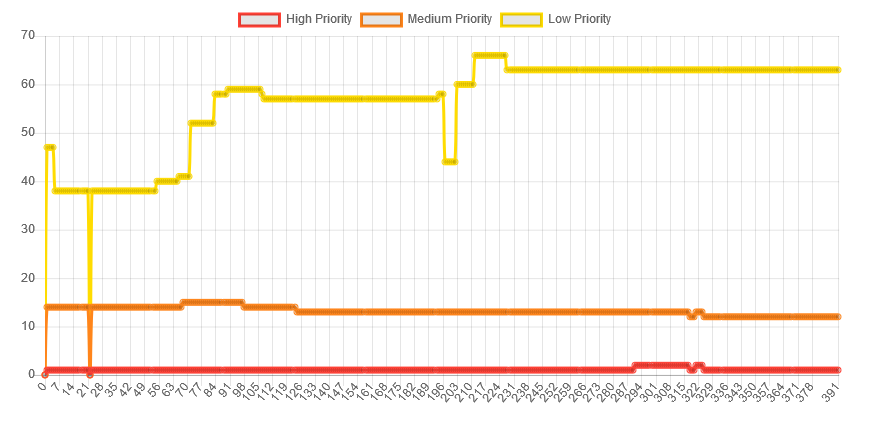
\includegraphics[width=\linewidth]{images/collections_td_timeline.png}
		\caption{Commons Collections}
		\label{fig:collections-td-timeline}
	\end{subfigure}
	\begin{subfigure}{.45\textwidth}
		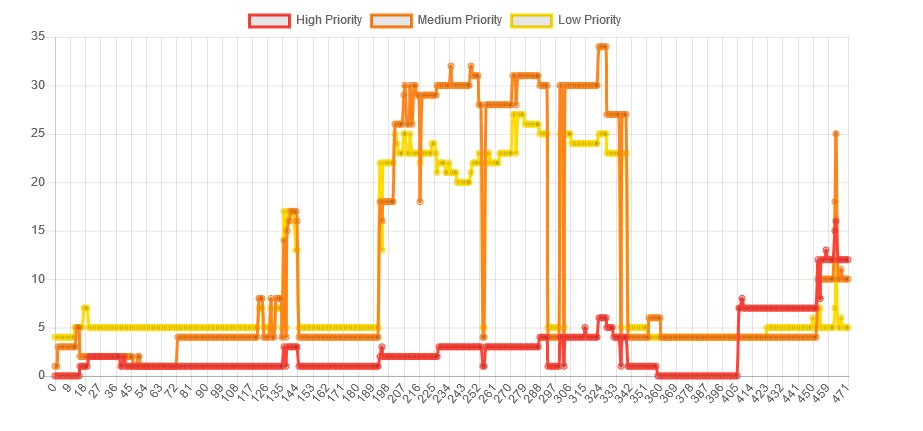
\includegraphics[width=\linewidth]{images/spring_td_timeline.png}
		\caption{Spring HATEOAS}
		\label{fig:spring-td-timeline}
	\end{subfigure}
	\caption{Technical Debt Timeline Comparison}
	\label{fig:td-timeline}
\end{figure*}

The relationship between total technical debt and both work effort calculations
can be seen in figure \ref{fig:td-total-debt}, for the \emph{Checkstyle}
project. Unfortunately the results do not show any meaningful pattern since
technical debt has remained more or less constant throughout project evolutions.
The two subfigures \ref{fig:td-total-debt-commit} and
\ref{fig:td-total-debt-ticket} appear to have a different population count,
possibly due to the difference in the statistics of work effort, mapped on the
\emph{x} axis. For work effort calculated using commit timestamps, the data
points are overlapping when values for effort are in the range $[0-10]$ whereas
data points are spread out for calculatins using ticket timestamps. The results
for the other projects show the exact same constant pattern. 

\begin{figure*}
	\centering
	\begin{subfigure}{.45\textwidth}
		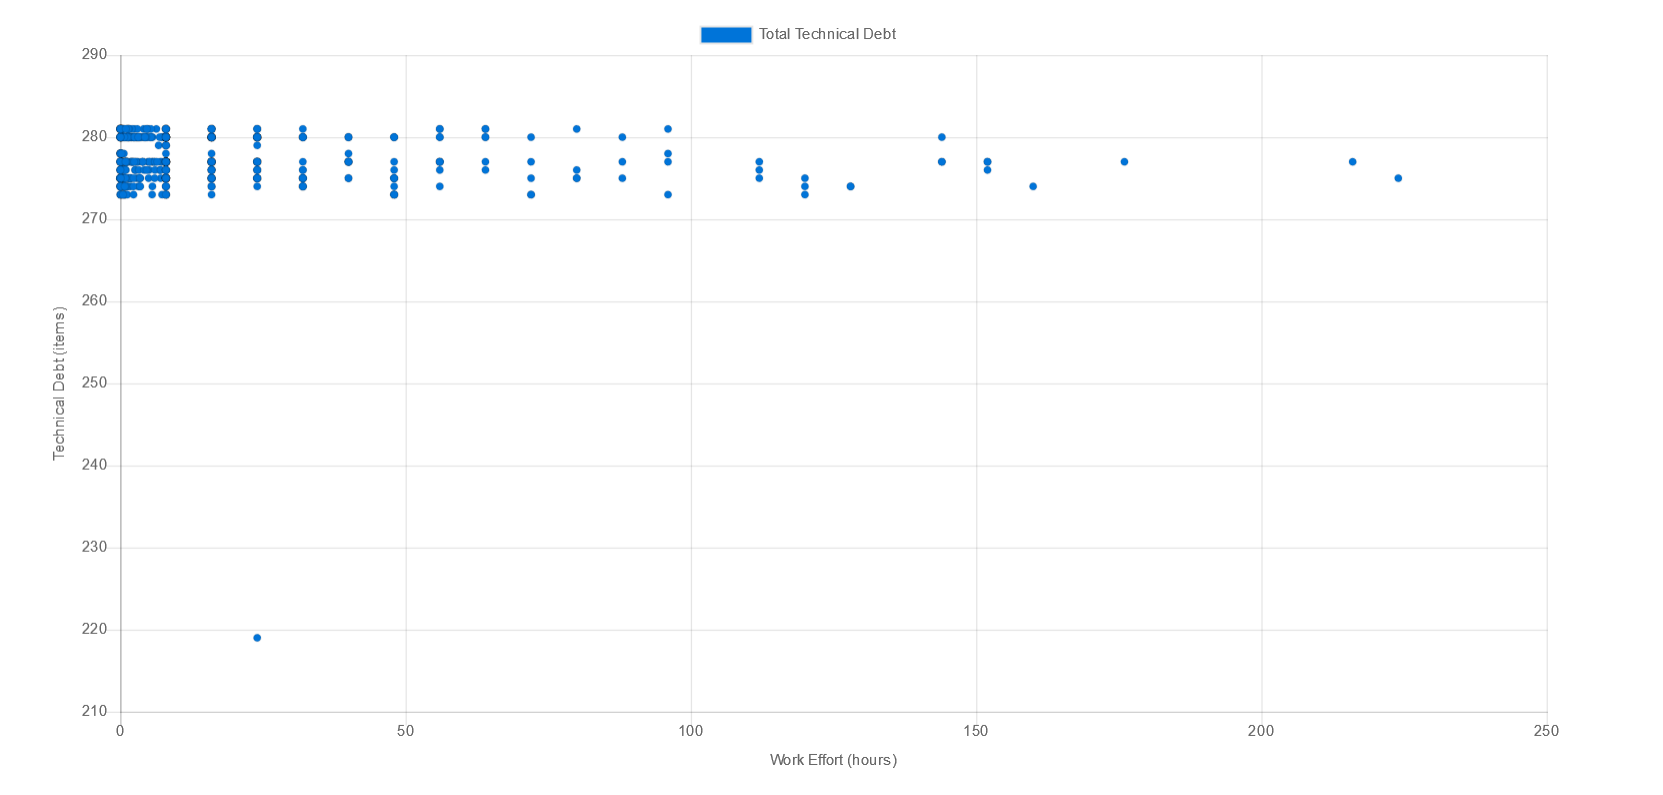
\includegraphics[width=\linewidth]{images/checkstyle_total_debt_commit.png}
		\caption{By Commit Timestamps}
		\label{fig:td-total-debt-commit}
	\end{subfigure}
	\begin{subfigure}{.45\textwidth}
		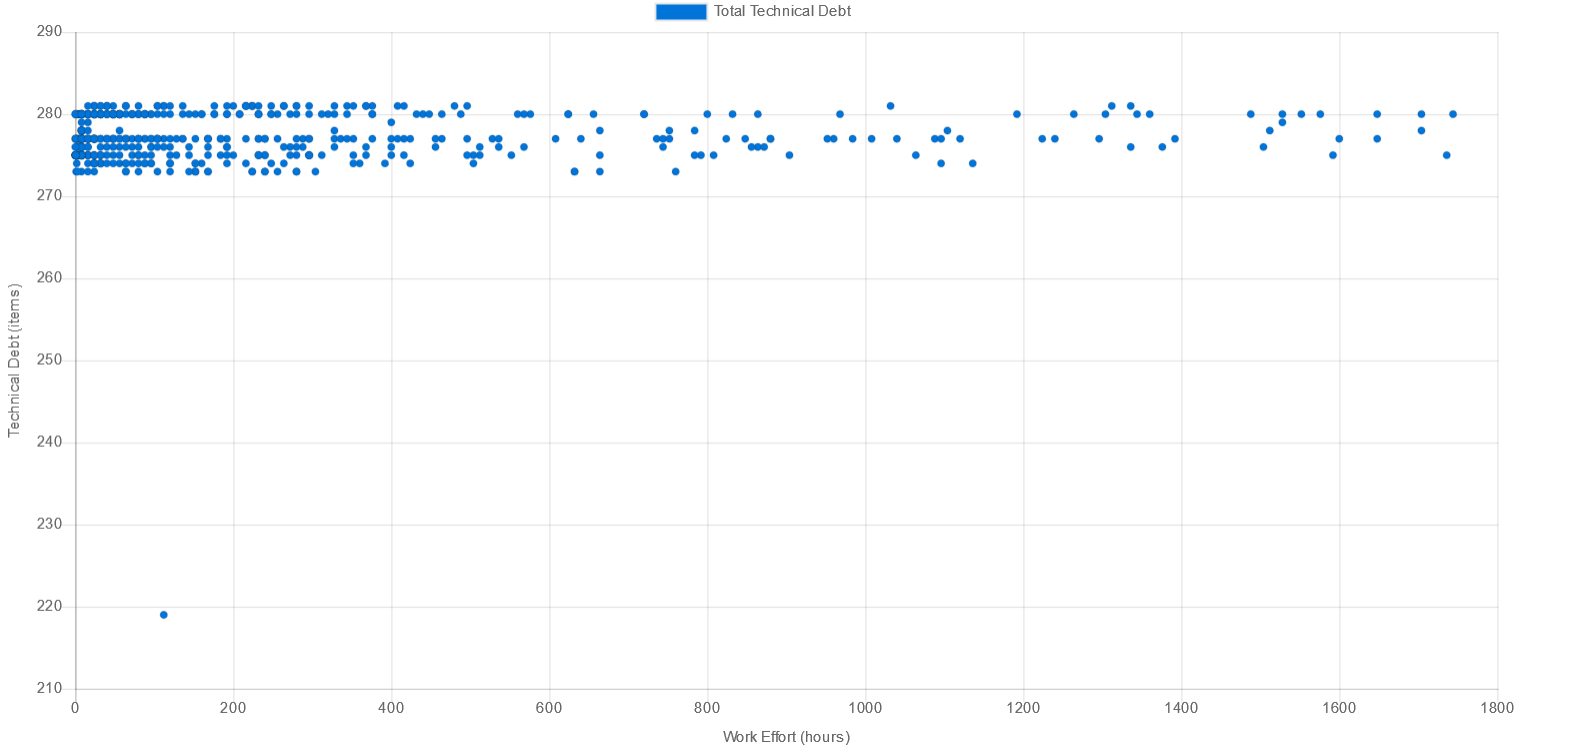
\includegraphics[width=\linewidth]{images/checkstyle_total_debt_ticket.png}
		\caption{By Ticket Timestamps}
		\label{fig:td-total-debt-ticket}
	\end{subfigure}
	\caption{Total Technical Debt and Work Effort for Checkstyle}
	\label{fig:td-total-debt}
\end{figure*}

Unfortunately, since technical debt is constant at the project level, the
relationship with work effort looks constant. This is most likely due to
consideration of quality at the project level, which may not affect the
productivity at the class level. 

% - - - - - - - - - - - - - - - - - - - - - - - - - - - - - - - - - - - - - - -
\subsubsection*{Experiment 2}
\label{experiment-2}

Since the results of experiment 1 are inconclusive, I decided to apply a
locality-based model for calculating technical debt. As mentioned in section
\ref{data-processing}, the locality model calculates technical debt based on the
change-set of each work task. Only code violations that are in the set of class
changes made by a developer are considered to affect the effort required to
accomplish the task. The statistics can be seen in figure
\ref{tab-technical-debt-local}.

\begin{table*}
	\centering
	\begin{tabular}{ |c|c|r|r|r|r|r| }
		\hline
		\multicolumn{2}{ |c| }{Category}                        & \emph{ANTLR} & \emph{Spring HATEOAS} & \emph{Checkstyle} & \emph{Commons Collections} & \emph{Commons Lang} \\ \hline \hline
		\multicolumn{1}{ |c  }{\multirow{2}{*}{TD Local Pain} } &
		\multicolumn{1}{ |l| }{Mean}                            & 1.814        & 0.34                  & 0.16              & 1.13                       & 6.299               \\ \cline{2-7}
		\multicolumn{1}{ |c  }{}                                &
		\multicolumn{1}{ |l| }{Std}                             & 7.861        & 1.205                 & 0.651             & 3.53                       & 13.635              \\ \cline{1-7}
	\end{tabular}
	\caption{\label{tab-technical-debt-local} Experiment 2: Technical Debt Statistics}
\end{table*}

When comparing to the total technical debt calculated in experiment 1, the
results have reduced dramatically. Although the same population of work items
has been used for both experiments, it seems that for the majority of projects,
very few technical debt issues on average affect the daily work of a developer.
This is surprising, especially since ANTLR had on average the most quality
issues out of all the projects. One factor which might influence the results is
the application domain of each project. A possible explanation for ANTLR is
that, because the project is a language generation tool, many files of its
source code could be language grammar files. Thus it is possible that many work
items revolve around changes to these files, which could not be analysed for
quality issues by FindBugs. 

\begin{figure*}
	\centering
	\begin{subfigure}{.45\textwidth}
		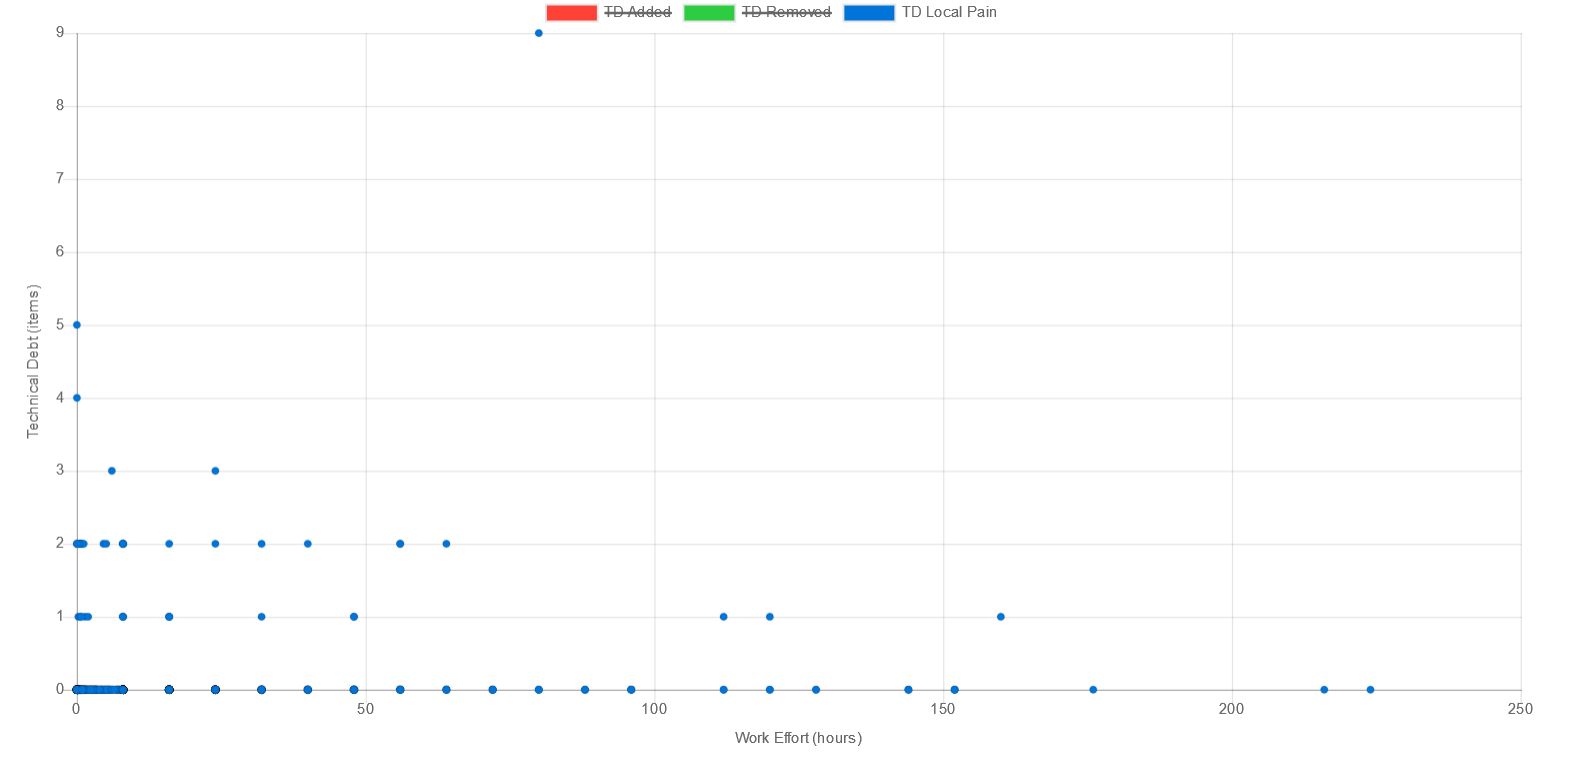
\includegraphics[width=\linewidth]{images/checkstyle_local_debt_commit.png}
		\caption{By Commit Timestamp}
		\label{fig:collections-td-timeline}
	\end{subfigure}
	\begin{subfigure}{.45\textwidth}
		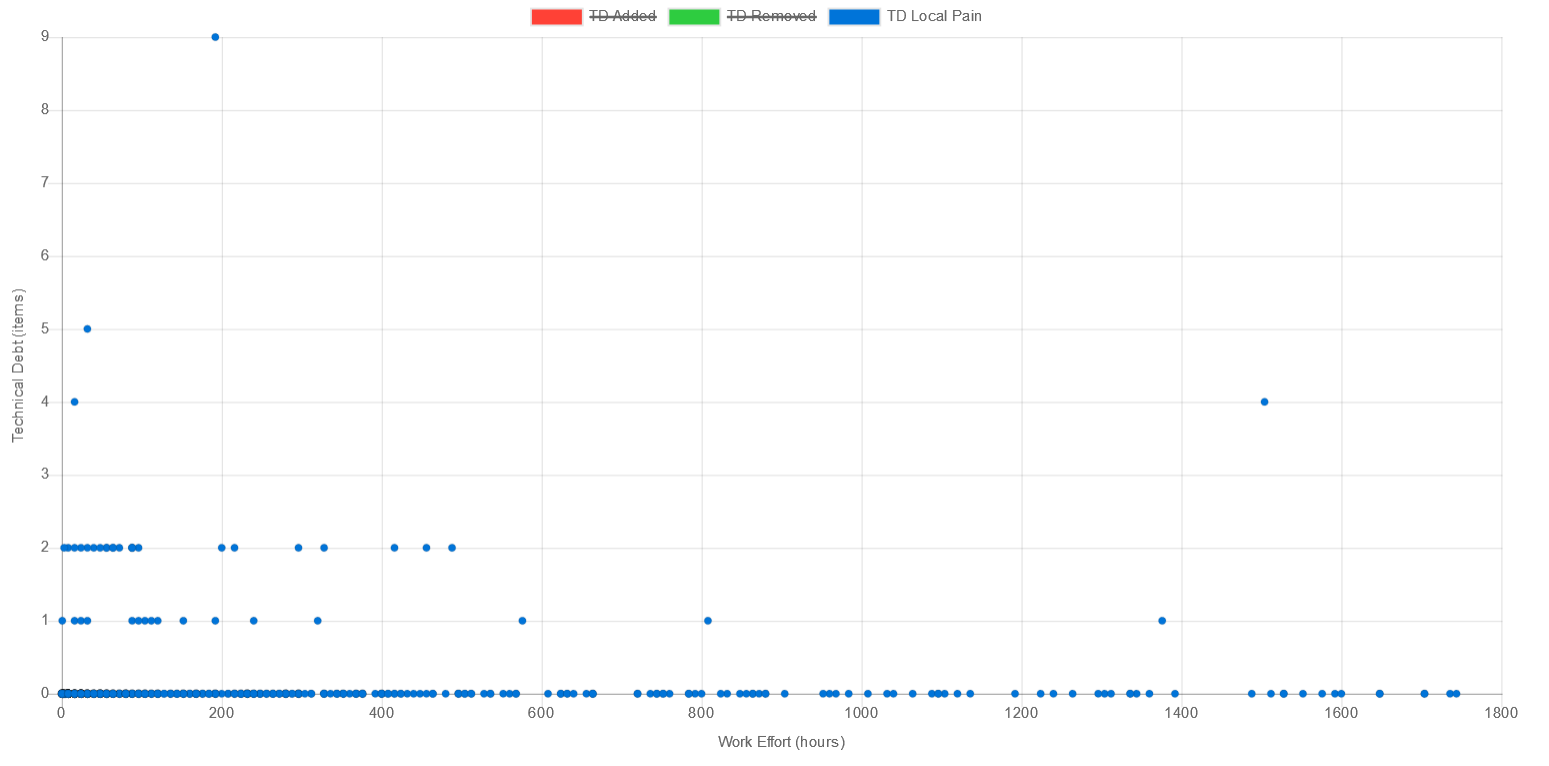
\includegraphics[width=\linewidth]{images/checkstyle_local_debt_ticket.png}
		\caption{By Ticket Timestamp}
		\label{fig:spring-td-timeline}
	\end{subfigure}
	\caption{Local Technical Debt and Work Effort for Checkstyle}
	\label{fig:td-local-debt}
\end{figure*}

The relationship between local technical debt and work effort per task can be
seen in figure \ref{fig:td-local-debt}, for \emph{Checkstyle}. The results seem
to have spread out, since technical debt is not as constant due to the change in
``level'' where technical debt items are considered to affect work. Similar to
\ref{fig:td-total-debt}, data points for the commit timestamp method are
concentrated in the range $[0-10]$ hours on the work effort axis due to the
calculations. On the other hand, they are spread out for the ticket method due
to the high variance of work effort previously calculated. The pattern by all
projects is exactly the same. There are many data points that are unaffected by
quality issues found and even the number of issues found do not vary as much as
expected. One possibility is that work items include very small changes to
classes that are unaffected by debt. Another possibility is that types of
quality issues found by the static analysis tools at the code level are not as
severe as those at the architectural level. I propose further research on the
topic in section \ref{future-work}. 

\begin{table*}
	\centering
	\begin{tabular}{ |c|c|r|r|r|r|r| }
		\hline
		\multicolumn{2}{ |c| }{Category}                        & \emph{ANTLR} & \emph{Spring HATEOAS} & \emph{Checkstyle} & \emph{Commons Collections} & \emph{Commons Lang} \\ \hline \hline
		\multicolumn{1}{ |c  }{\multirow{2}{*}{TD Added} }      &
		\multicolumn{1}{ |l| }{Mean}                            & 40.561       & 0.325                 & 4.814             & 3.493                      & 4.918               \\ \cline{2-7}
		\multicolumn{1}{ |c  }{}                                &
		\multicolumn{1}{ |l| }{Std}                             & 168.236      & 1.49                  & 19.525            & 10.196                     & 16.139              \\ \cline{1-7}

		\multicolumn{1}{ |c  }{\multirow{2}{*}{TD Removed} }    &
		\multicolumn{1}{ |l| }{Mean}                            & 50.598       & 1.593                 & 4.966             & 1.768                      & 4.392               \\ \cline{2-7}
		\multicolumn{1}{ |c  }{}                                &
		\multicolumn{1}{ |l| }{Std}                             & 190.364      & 7.432                 & 19.846            & 5.486                      & 14.605              \\ \cline{1-7}
	\end{tabular}
	\caption{\label{tab-technical-debt-intro} Experiment 3: Technical Debt Statistics}
\end{table*}

% - - - - - - - - - - - - - - - - - - - - - - - - - - - - - - - - - - - - - - -
\subsubsection*{Experiment 3}
\label{experiment-3}

Lastly, for the third experiment, I wanted to check if the number of technical
debt items added might reduce the effort needed to complete a task. Similarly, I
wanted to study whether removal of quality issues would increase the work
effort, possibly through refactoring activities. The initial statistics for
technical debt introduced and removed can be seen in table
\ref{tab-technical-debt-intro}. 

\begin{figure*}
	\centering
	\begin{subfigure}{.45\textwidth}
		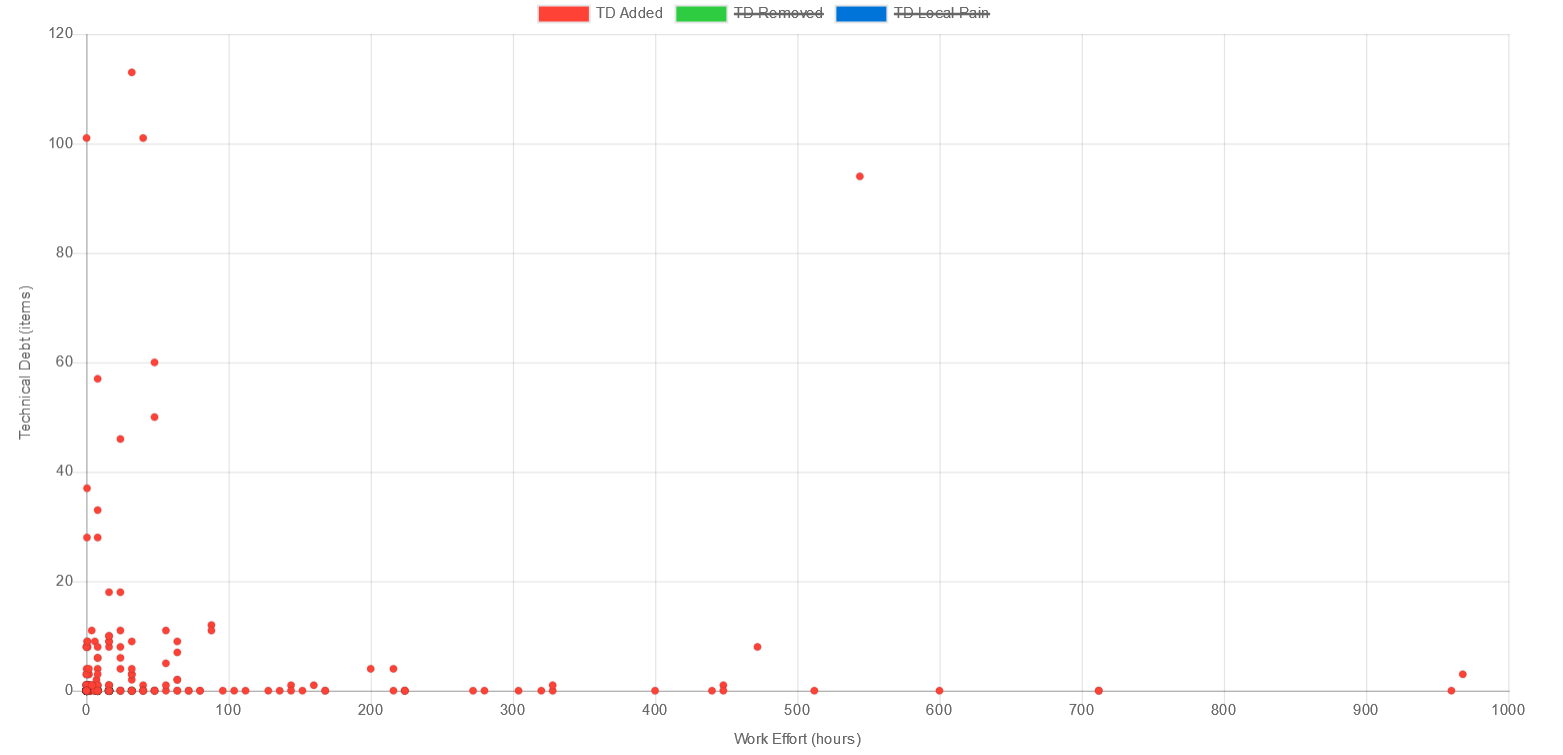
\includegraphics[width=\linewidth]{images/collections_added_debt_commit.png}
		\caption{Total Technical Debt}
		\label{fig:td-added-commit}
	\end{subfigure}
	\begin{subfigure}{.45\textwidth}
		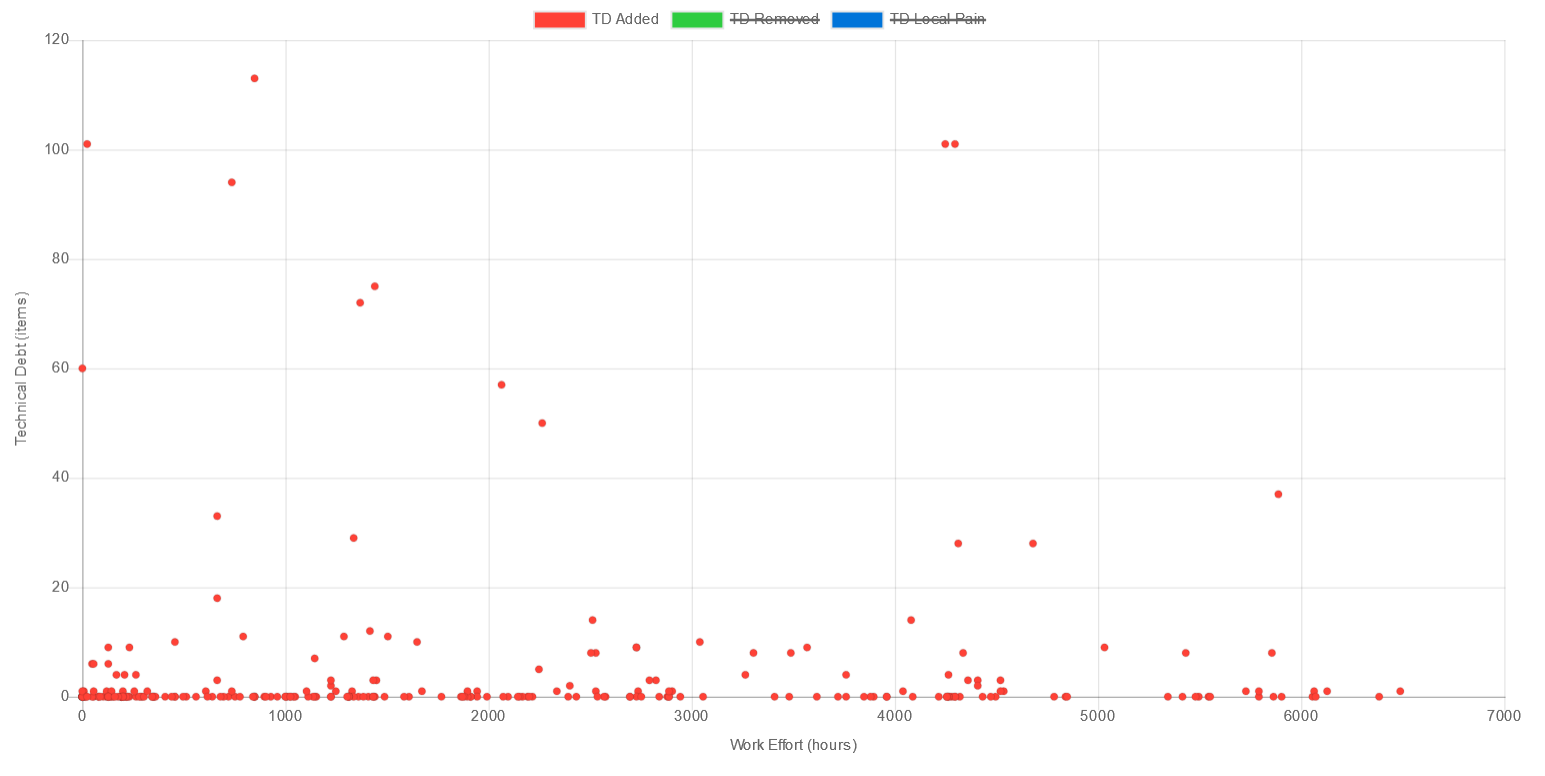
\includegraphics[width=\linewidth]{images/collections_added_debt_ticket.png}
		\caption{Local Technical Debt}
		\label{fig:td-added-ticket}
	\end{subfigure}
	\caption{Technical Debt Added and Work Effort for Collections}
	\label{fig:td-added}
\end{figure*}


It seems that, on average, \emph{ANTLR} has many introductions and removals of
debt items. The developers of \emph{Spring HATEOAS}, since it is a younger
project, are focusing on removal of quality issues to eliminate the threats of
bugs that a new project may be prone to. The other projects have very similar
results for both sets of calculations. It seems that, on average, the number of
quality issues introduced by work items is approximately equal to the number of
technical debt items removed. This might be a consequence of adding new features
with initial quality issues which are refined over time by the team through
other tasks such as fixing bugs and other refactoring activities.

\begin{figure*}
	\centering
	\begin{subfigure}{.45\textwidth}
		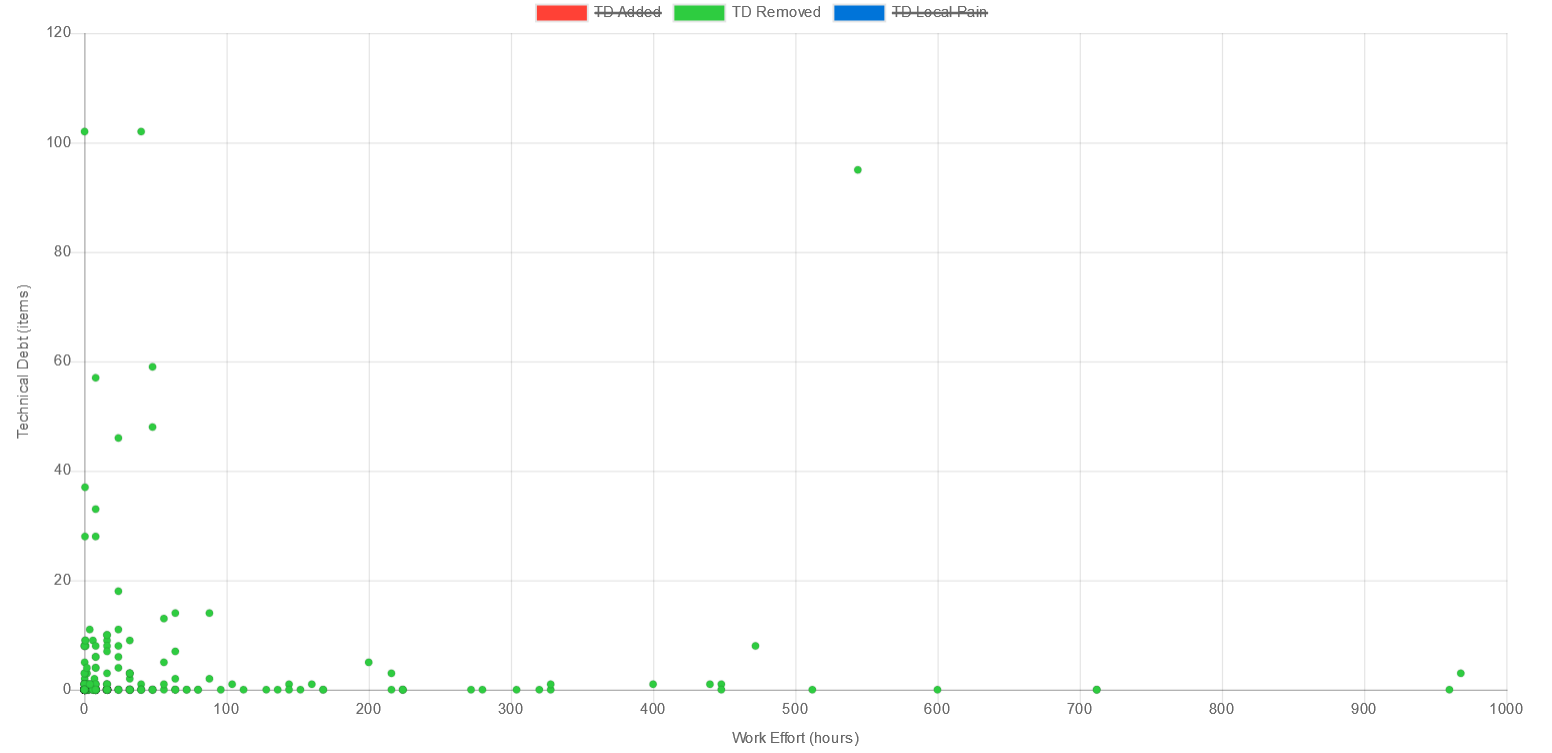
\includegraphics[width=\linewidth]{images/collections_removed_debt_commit.png}
		\caption{By Commit}
		\label{fig:td-removed-commit}
	\end{subfigure}
	\begin{subfigure}{.45\textwidth}
		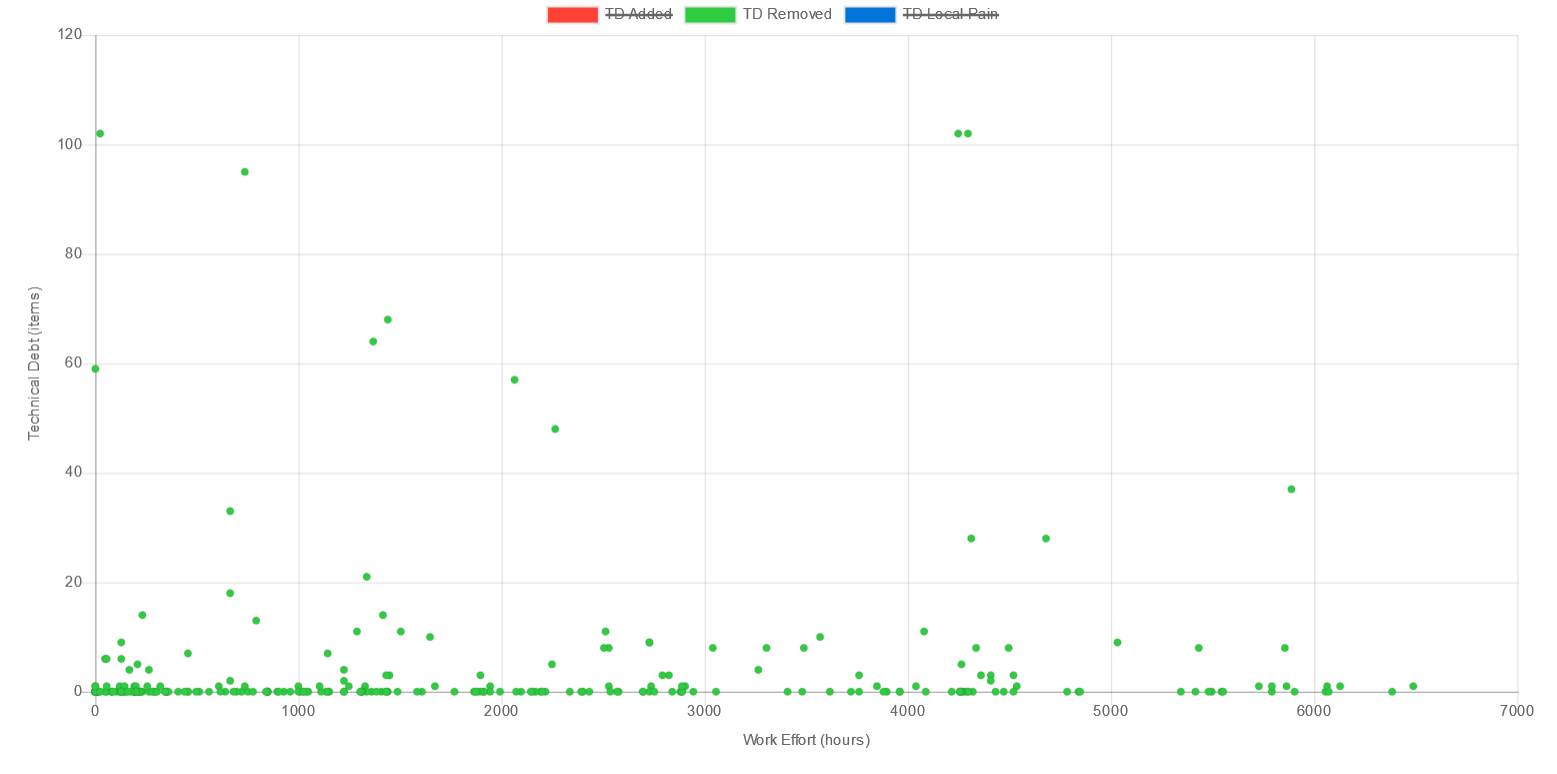
\includegraphics[width=\linewidth]{images/collections_removed_debt_ticket.png}
		\caption{By Ticket}
		\label{fig:td-removed-ticket}
	\end{subfigure}
	\caption{Technical Debt Removed and Work Effort for Collections}
	\label{fig:td-removed}
\end{figure*}

Lastly, the relationship between work effort calculations and technical debt
added and removed are presented in figures \ref{fig:td-added} and
\ref{fig:td-removed}, respectively. The four figures display similar patterns to
the previous local debt relationship with work effort, presented in figure
\ref{fig:td-local-debt}. It seems that as work effort increases, technical debt
decreases. This observation makes sense for removal of technical debt since work
effort should increase with refactoring activities. However, the distribution of
data points are mostly around the range $[0-100]$ hours on the work effort axis.
The pattern is shared by the work effort and TD added relationship, which is the
opposite of my initial expectation. \\


Although the three experiments build on one another, from my perspective there
is no correlation between work effort and technical debt. The first experiment
showed that technical debt at the project level does affect the effort required
to finish tasks. Additionally, the relationship between work effort and local
technical debt follows a negative pattern, since increase in work effort shows
that technical debt decreases. This pattern is shared by the results of the
third experiment. I consider the results to be inconclusive due to many factors
being controlled for the simplicity of the calculations.

%%%%%%%%%%%%%%%%%%%%%%%%%%%%%%%%%%%%%%%%%%%%%%%%%%%%%%%%%%%%%%%%%%%%%%%%%%%%%%%
%%%%%%%%%%%%%%%%%%%%%%%%%%%%%%%%%%%%%%%%%%%%%%%%%%%%%%%%%%%%%%%%%%%%%%%%%%%%%%%
%%%%%%%%%%%%%%%%%%%%%%%%%%%%%%%%%%%%%%%%%%%%%%%%%%%%%%%%%%%%%%%%%%%%%%%%%%%%%%%
\section{Validity and Future Work}
\label{validity-future-work}

Throughout the study, there have been numerous simplifying assumptions that may
cripple the results and conclusion presented in the earlier section. These range
from each type of calculation and from other subjective factors that are
difficult to model in such a short experiment. The omitted factors are
considered here as well as future work for proceeding experiments.

%%%%%%%%%%%%%%%%%%%%%%%%%%%%%%%%%%%%%%%%%%%%%%%%%%%%%%%%%%%%%%%%%%%%%%%%%%%%%%%
\subsection{Threaths to Validity}
\label{validity}

% - - - - - - - - - - - - - - - - - - - - - - - - - - - - - - - - - - - - - - -
\subsubsection*{Work Effort Measurement}
\label{validity-work}

There are a number of simplifying assumptions that have been made in the design
process of the work calculation methods. Although such assumptions simplify the
method of computation, it additionally `curves' the results. The following
factors may have had an impact on the computed results:

\begin{enumerate}
  \item We considered work to have a `linear' pattern. That is, only one
  developer per work item and once the task is accomplished, the developer
  directly starts a new task. This is not always the case since developers may
  collaborate on tasks. This is reflected in the calculation using commit
  timestamps. 
  \item We considered that a developer works on a single item at a time. This
  may not be true. In corporate and open-source environments, it is very likely
  that engineers work on multiple items at at time.  
  \item We did not introduce external workflow variables such as mini breaks for
  coffee, meetings or time off. This means that work effort results may contain
  non-development time. 
  \item We considered that developers work continously, on 8 hours per day. This
  might not be accurate, especially in open-source projects. Engineers might
  take less time out of their schedule if they are working on a part time basis.
  \item Additionally, factors such as technical experience, knowledge of the system,
  familiarity with libraries and dependencies used, personality and intrinsic
  complex details of the work involved have not been considered in the
  calculation. Collecting such data means tracking down and interviewing each
  project collaborator. Moreover, modelling such subjective factors in work effort
  is a complex challenge. 
\end{enumerate}

% - - - - - - - - - - - - - - - - - - - - - - - - - - - - - - - - - - - - - - -
\subsubsection*{Technical Debt Measurement}
\label{validity-td}

Similarly, for technical debt calculations some simplifying assumptions were
introduced to reduce the complexity of measurement:

\begin{enumerate}
  \item The technical debt measurement is a simple count of all quality issues
  found per revision. Severity of the quality issues was not considered.
  \item The data collection phase only analysed the source code for simple code
  bug patterns. Testing or architectural debt were not considered. 
  \item There are other types of technical debt \emph{REFERENCE} which have not
  been considered due to complexity in the modelling of such factors. For
  example, requirements debt \emph{REFERENCE} takes more effort out of a
  developer's time.
\end{enumerate}

Although these assumptions are simplific they have been added for this purpose.
Due to the nature of the variables involved, it is difficult to model specific
factors into the computations without supporting data. Therefore, we hope that
this experiment will be the starting point for further research in this area. 

%%%%%%%%%%%%%%%%%%%%%%%%%%%%%%%%%%%%%%%%%%%%%%%%%%%%%%%%%%%%%%%%%%%%%%%%%%%%%%%
\subsection{Future Work}
\label{future-work}

The results shown require a few changes to the underlying computation methods
for work effort and technical debt accuracy. First of all, a more complex
identification mechanism and computation of technical debt measurement should be
considered. There is value in identifying quality issues at the test and
architecture level for various modules of projects and see how these may affect
work effort in comparison with code debt. Many methods \emph{REFERENCE}
\emph{REFERENCE} have been devised for measuring technical debt that could be
tailored for analysing debt items for each revision and work item.

Work effort methods could be improved by gathering more data on the teams and
collaborators of each project through interviews and questionnaires. This would
command a greater understanding of development patterns and provide additional
data to the computation and validation of work effort.

Additional experiments may expand on the data collected from the project
management tool. For example, it would be interesting if there is any
correlation between tickets types such as features, enhacements, bugs and
others. Moreover, ticket complexity plays a great role in assessing an initial
work effort and would an interesting to note how technical debt affects the
actual work effort in relation to the early estimation. Additional expansions of
this experiment would also look at ticket priority and how technical debt varies
between the starting and ending revision of such a work item. 

Lastly, it would be beneficial to expand the number of candidates and include a
varied set of domains, languages, version control systems and project management
tools.

%%%%%%%%%%%%%%%%%%%%%%%%%%%%%%%%%%%%%%%%%%%%%%%%%%%%%%%%%%%%%%%%%%%%%%%%%%%%%%%
%%%%%%%%%%%%%%%%%%%%%%%%%%%%%%%%%%%%%%%%%%%%%%%%%%%%%%%%%%%%%%%%%%%%%%%%%%%%%%%
%%%%%%%%%%%%%%%%%%%%%%%%%%%%%%%%%%%%%%%%%%%%%%%%%%%%%%%%%%%%%%%%%%%%%%%%%%%%%%%
\section{Conclusion}
\label{conclusion}

%%%%%%%%%%%%%%%%%%%%%%%%%%%%%%%%%%%%%%%%%%%%%%%%%%%%%%%%%%%%%%%%%%%%%%%%%%%%%%%
%%%%%%%%%%%%%%%%%%%%%%%%%%%%%%%%%%%%%%%%%%%%%%%%%%%%%%%%%%%%%%%%%%%%%%%%%%%%%%%
%%%%%%%%%%%%%%%%%%%%%%%%%%%%%%%%%%%%%%%%%%%%%%%%%%%%%%%%%%%%%%%%%%%%%%%%%%%%%%%
{\bf Acknowledgments.} This is optional; it is a location for you to thank
people

\bibliographystyle{abbrv}
\bibliography{mdiss}

\end{document}